% Single-column draft. Build:  pdflatex main && bibtex main && pdflatex main && pdflatex main
% Figures are produced by paper/make_figures.py from paper/data/paper_data.json.
\documentclass[11pt,a4paper]{article}

\usepackage[margin=1in]{geometry}
\usepackage{graphicx}
\usepackage{booktabs}
\usepackage{amsmath}
\usepackage{amssymb}
\usepackage{caption}
\usepackage{subcaption}
\usepackage{microtype}
\usepackage[table]{xcolor}
\usepackage{multirow}
\usepackage[hidelinks]{hyperref}
\usepackage{natbib}

\captionsetup{font=small,labelfont=bf,skip=6pt}
\newcommand{\eer}{\textsc{eer}}
\newcommand{\mindcf}{\textsc{minDCF}}
\newcommand{\best}[1]{\textbf{#1}}

\title{\bf Diversity Without Difference: Why Architectural Variation Fails to
Produce Fusable Speech Deepfake Detectors, and Why the Development Set
Cannot Tell You}

\author{A.\ Harisha\\[2pt]
\small Sahyadri College of Engineering and Management\\
\small \texttt{harisha@sahyadri.edu.in}}

\date{\today}

\begin{document}
\maketitle

\begin{abstract}
\noindent
Fusing several countermeasures is the standard route to strong speech deepfake detection, and the
winning ASVspoof~5 system fuses twelve.
We ask what the members of such a fusion must actually differ in, and find that architectural
variation is not enough: four detectors built on one self-supervised backbone but differing in
pooling, representation, topology and even backbone behave as \emph{1.10 independent systems} out
of four, with the leading principal component carrying 95.5\% of the score variance.
We build each detector identically apart from its back-end, measure the eigen-spectrum of their
score correlation, and evaluate on the ASVspoof~5 evaluation set and on an out-of-domain
in-the-wild set.
Only a change of \emph{view}---replacing time-mean pooling with attention over frames---moved the
correlation at all ($0.994 \rightarrow 0.917$), and our selected two-member system reaches
\best{3.21\%} \eer{} / \best{0.0905} \mindcf{}, ahead of the other published open-condition system
we could verify (4.04\%) and short of the 2.59\% twelve-system winner.
Two further results cut against common practice: the ASVspoof~5 development split cannot rank these
systems (Spearman $\rho = +0.01$, rising only to $+0.24$ when a neural-codec view is added), so our
protocol selects a system 0.28~\eer{} points worse than the best in our own pool; and the
best in-domain member is the \emph{worst} out of domain, with every system degrading by a factor of
2.5--3.8 on found audio.
\end{abstract}

\section{Introduction}

Speech deepfake detection is evaluated almost entirely in domain. A countermeasure is trained on one
corpus, selected on that corpus's development split, and reported on its evaluation set; the
leaderboard orders systems by a single pooled equal error rate. Fusion of several countermeasures is
the standard way to the top of such a leaderboard, and the winning ASVspoof~5 open-condition system
fuses twelve single systems across three back-end families \citep{ustc2024}.

This paper asks a narrower question than ``how do we win'': \emph{what must fusion members differ in
for fusion to pay?} We build four detectors that share a training corpus, a frozen self-supervised
backbone, an adaptation scheme, an augmentation policy, a seed and a schedule, and differ only in
their back-end---time-mean pooling, attentive pooling, a hand-crafted cepstral branch, and graph
attention---plus a fifth varying the backbone itself. We then measure not just whether they fuse,
but \emph{how many independent systems they amount to}.

The answer is uncomfortable. Across three architectural axes and two backbones, the four members
behave as \textbf{1.10 effective systems out of four}. Their first principal component explains
95.5\% of the score variance and loads within 0.006 of $0.50$ on every member: they are, in
information terms, one system wearing four hats. The only intervention that moved the number was a
change of \emph{view}---opening the time axis that time-mean pooling discards---and the 0.10~\eer{}
points it bought came from 3.2\% of the variance.

We report three further findings, each of which complicates the leaderboard reading of this task.

\begin{enumerate}\itemsep2pt
\item \textbf{The development split cannot select these systems.} ASVspoof~5's train and development
partitions are 100\% uncoded while 75\% of the evaluation set is coded. Over all 15 member subsets,
the rank correlation between development and evaluation \eer{} is $\rho = +0.011$ ($p=0.97$). Adding
a neural-codec development view raises it only to $+0.236$ ($p=0.40$). Our protocol therefore selects
a system 0.28~\eer{} points worse than the best in our pool, and we report both numbers.
\item \textbf{In-domain rank inverts out of domain.} On an in-the-wild set, our best in-domain
member is the worst, and our third-best is the best by a wide margin. All systems degrade by
2.5--3.8$\times$.
\item \textbf{The evaluation set is smaller than it looks.} Its 680{,}774 clips derive from 171{,}602
source utterances, each appearing clean plus roughly three codec variants. Bootstrap intervals that
resample clips---ours in earlier drafts, and, we suspect, most reported on this corpus---are about
$2\times$ too narrow.
\end{enumerate}

\section{Related work}

Self-supervised speech representations are the dominant front end for this task. We use
WavLM-Large \citep{wavlm}; XLS-R \citep{xlsr} is our second backbone. Low-rank adaptation
\citep{lora} lets us fine-tune a 300M-parameter backbone with 3.15M trainable parameters.

On back-ends, AASIST \citep{aasist} introduced heterogeneous spectro-temporal graph attention and is
the architecture family our graph member is derived from; we reuse its graph attention layer but not
its heterogeneous cross-attention or master node, and we are explicit that our variant is not AASIST.
Attentive pooling over frozen SSL layers, and automatic layer selection, are studied by
\citet{serrano2025}, who also report that score-level fusion of several encoders improves
out-of-domain generalisation.

For augmentation we use RawBoost \citep{rawboost} and simulated codecs, and we add the neural codec
EnCodec \citep{encodec} during training. The adversarial attacks present in the ASVspoof~5 evaluation
set are Malafide \citep{malafide} and Malacopula \citep{malacopula}.

Our comparison points on ASVspoof~5 track~1 are the challenge overview \citep{asvspoof5}, the winning
USTC-KXDIGIT system at 2.59\% \eer{} / 0.0750 \mindcf{} in the open condition \citep{ustc2024}, and
SZU-AFS at 4.04\% / 0.115 \citep{szuafs}. Both report on the full evaluation set under the official
cost model, as we do.

\section{Data}
\label{sec:data}

\begin{table}[t]
\centering
\small
\caption{Corpora. ASVspoof~5 attack sets are disjoint across partitions, so every reported number is
on unseen spoofing systems. Train and development are entirely uncoded; 75\% of the evaluation set
carries one of eleven real codecs.}
\label{tab:data}
\begin{tabular}{lrrrrl}
\toprule
Partition & Clips & Bona fide & Speakers & Attacks & Channel \\
\midrule
ASVspoof~5 train & 182{,}357 & 18{,}797 (10.3\%) & 400 & A01--A08 & uncoded \\
ASVspoof~5 dev   & 140{,}950 & 31{,}334 (22.2\%) & 785 & A09--A16 & uncoded \\
ASVspoof~5 eval  & 680{,}774 & 138{,}688 (20.4\%) & 737 & A17--A32 & clean + C01--C11 \\
In-the-Wild      & 31{,}779  & 19{,}963 (62.8\%) & 54  & unlabelled & unknown \\
\bottomrule
\end{tabular}
\end{table}

Table~\ref{tab:data} and Figure~\ref{fig:dataset} describe the corpora. Three properties of
ASVspoof~5 \citep{asvspoof5} drive everything that follows.

\textbf{Disjoint attacks.} A01--A08, A09--A16 and A17--A32 do not overlap, so a system is always
tested on spoofing algorithms it has never seen. This design repeatedly caught training-attack
memorisation in our own runs that training loss hid completely.

\textbf{A channel mismatch between selection and test.} Train and development are uncoded. The
evaluation set is 75\% coded, with eleven conditions. We simulate ten of the eleven during training;
only C11 (device variation) is never simulated. Section~\ref{sec:selection} shows that this
mismatch, and not any property of the models, is what breaks model selection.

\textbf{A source-utterance structure that inflates the apparent sample size.} Every coded evaluation
clip carries a \texttt{CODEC\_SEED} pointing at its original, and all 509{,}172 coded clips have
their original also present. The 680{,}774 clips therefore come from \textbf{171{,}602 source
utterances}, a mean of 3.97 clips per source. Treating clips as independent in a bootstrap
understates every interval by roughly $\sqrt{4}$. Intervals in this paper are computed with a
clustered bootstrap over source utterances.

In-the-Wild is used for reporting only; nothing is selected or calibrated on it. Note its inverted
class prior (62.8\% bona fide), which makes \mindcf{} under the official 0.05 spoof prior
incomparable with the ASVspoof numbers; we report \eer{} there.

\begin{figure}[t]
\centering
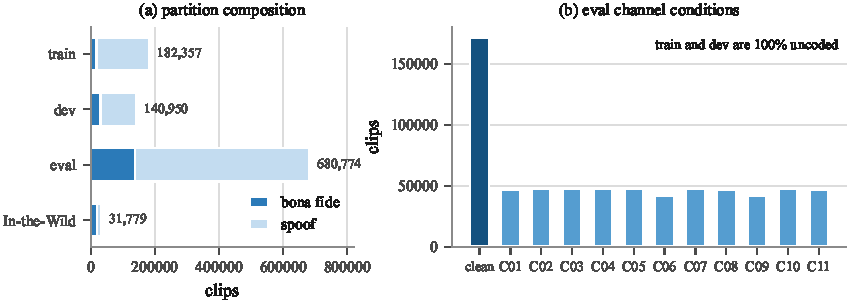
\includegraphics[width=\textwidth]{figures/fig10_dataset}
\caption{(a) Partition composition. (b) Evaluation-set channel conditions. The selection split
contains none of the eleven coded conditions the evaluation set is judged on.}
\label{fig:dataset}
\end{figure}

\section{Systems}

\begin{figure}[t]
\centering
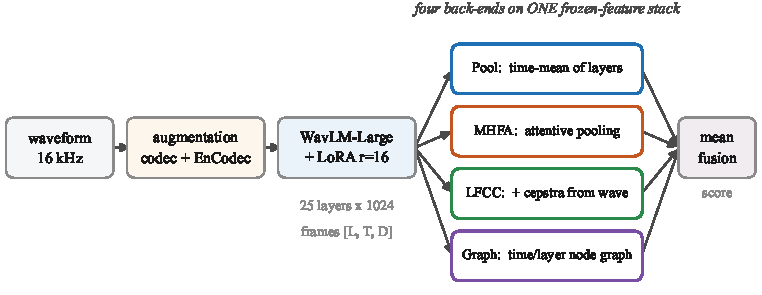
\includegraphics[width=\textwidth]{figures/fig1_architecture}
\caption{All four members share the waveform pipeline, the augmentation policy and the adapted
WavLM-Large backbone, and differ only in the back-end that turns per-layer frames into a score.}
\label{fig:arch}
\end{figure}

Figure~\ref{fig:arch} shows the common pipeline. A waveform is augmented, then passed through
WavLM-Large \citep{wavlm} adapted with LoRA of rank 16 on the attention projections \citep{lora}
(3.15M trainable parameters). The backbone emits 25 layer activations. Augmentation applies one of
eight simulated codecs with probability 0.5 and, with probability 0.3, EnCodec \citep{encodec} on the
GPU---the neural codec corresponding to evaluation conditions C04 and C07, which the DataLoader
cannot apply because it requires a GPU.

The four back-ends are:

\textbf{Pool} (0.26M parameters) takes the time-\emph{mean} of each layer, learns a softmax weighting
over layers, and applies a two-layer MLP. This is the conventional design and the baseline for
everything else.

\textbf{MHFA} (0.53M) keeps the frames. It learns two \emph{separate} layer weightings---one
producing keys, one producing values---and pools over time by multi-head attention, so the layers
that decide \emph{where} to look need not be the layers carrying the evidence.

\textbf{LFCC} (0.50M) adds a second \emph{representation}: 20 linear-frequency cepstral coefficients
with first and second deltas, computed from the waveform and aligned frame-for-frame with the
backbone, concatenated with the frames before attentive pooling. Part of its evidence cannot
correlate with anything the backbone encodes.

\textbf{Graph} (0.30M) adds a second \emph{topology}: graph attention over two node sets, time slots
and backbone layers, reusing the graph attention layer of AASIST \citep{aasist}. It is not AASIST---
there is no heterogeneous cross-attention and no master node, and the spectral sub-graph is replaced
by a layer sub-graph because SSL frames have no frequency axis---and no result here should be read
under that name.

Members are combined by the unweighted mean of scores standardised on the development
\texttt{calib} split. The combiner has no parameters fit on evaluation data.

\section{Protocol}

Models are selected on the development \texttt{select} split (attacks A09--A16), scale statistics are
fit on the speaker-disjoint \texttt{calib} half, and the evaluation set is scored once. Metrics are
\eer{} and \mindcf{} under the official ASVspoof~5 cost model (spoof prior $0.05$, $C_\text{miss}=1$,
$C_\text{fa}=10$), plus $\text{min}C_\text{llr}$. Differences are tested with a paired bootstrap
clustered on source utterance (Section~\ref{sec:data}).

All members use seed 1337, batch size 32, eight epochs, head learning rate $10^{-3}$ and backbone
learning rate $10^{-5}$. \textbf{A limitation we state up front:} the members below are single-seed.
In earlier three-seed experiments on this codebase, frozen single models varied by 0.33~\eer{} points
across seeds---larger than the 0.10-point fusion gain we report. Seed variance for the systems in
Table~\ref{tab:members} is therefore \emph{unmeasured}, and the fusion gain should be read with that
in mind.

\section{Results}

\subsection{Members}

\begin{table}[t]
\centering
\small
\caption{The four members. All share everything but the back-end. Dev select is the mean \eer{} over
the clean and codec development views; in-the-wild is out-of-domain and reporting only.
$\rho_{\text{Pool}}$ is the Pearson correlation of evaluation scores with the Pool member.}
\label{tab:members}
\begin{tabular}{llrrrrrr}
\toprule
& & & \multicolumn{3}{c}{ASVspoof~5 eval} & \multicolumn{1}{c}{In-the-Wild} & \\
\cmidrule(lr){4-6}\cmidrule(lr){7-7}
Member & Back-end differs in & Dev sel. & \eer{} & \mindcf{} & min$C_\text{llr}$ & \eer{} & $\rho_{\text{Pool}}$ \\
\midrule
Pool  & ---                 & \best{1.50} & 3.31 & 0.0942 & 0.1256 & 11.25 & --- \\
MHFA  & pooling             & 2.07 & 3.44 & 0.0957 & 0.1286 & \best{8.51} & 0.917 \\
LFCC  & representation      & 2.95 & \best{3.11} & \best{0.0845} & \best{0.1164} & 11.82 & 0.965 \\
Graph & topology            & 3.10 & 3.93 & 0.1091 & 0.1475 & 11.44 & 0.943 \\
\bottomrule
\end{tabular}
\end{table}

Table~\ref{tab:members} is the central table of the paper, and almost every column disagrees with
every other. Pool is the best member on development and only third on evaluation. LFCC is the
\emph{worst} on development, the \emph{best} on evaluation, and the \emph{worst} again in the wild.
MHFA is third in domain and first out of domain by 2.7~points.

Figure~\ref{fig:curves} shows that these differences are not training artefacts: none of the members
shows the rising-development / falling-training signature of attack memorisation, and the LFCC member
simply peaks at epoch~1 and then slowly overfits. Figure~\ref{fig:det} gives the detection error
trade-off curves; the fused systems dominate the single members across the operating range, not only
at the equal error point.

\begin{figure}[t]
\centering
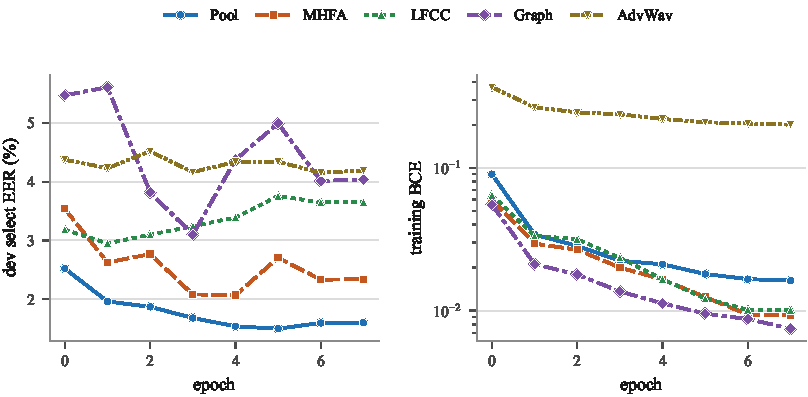
\includegraphics[width=\textwidth]{figures/fig2_training_curves}
\caption{Training behaviour. Left: development \eer{}. Right: training loss. AdvWav is the
adversarially trained model of Section~\ref{sec:robust}, still in progress at submission.}
\label{fig:curves}
\end{figure}

\begin{figure}[t]
\centering
\begin{minipage}{0.48\textwidth}
\centering
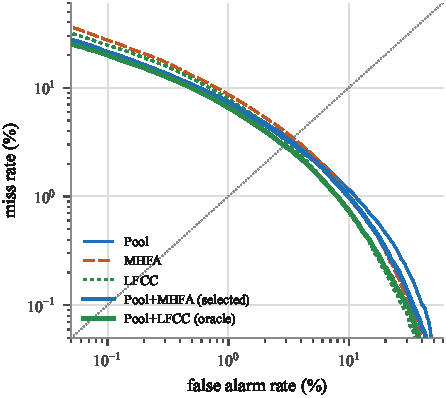
\includegraphics[width=\textwidth]{figures/fig3_det}
\end{minipage}\hfill
\begin{minipage}{0.48\textwidth}
\centering
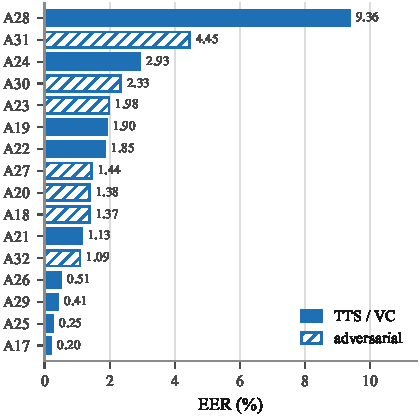
\includegraphics[width=\textwidth]{figures/fig5_per_attack}
\end{minipage}
\caption{Left: DET curves on the evaluation set; solid curves are fusions. Right: per-attack \eer{}
of the selected system. The pooled number is dominated by A28; nine of sixteen attacks sit below
1.5\%, and the adversarial attacks (hatched) are not the hard ones.}
\label{fig:det}
\end{figure}

\subsection{Conditions and attacks}

Figure~\ref{fig:codec} breaks the evaluation set down by channel. The two neural codecs, C04 and C07,
are by a wide margin the hardest conditions for every member---a direct consequence of their absence
from any uncoded training view before we added GPU-side EnCodec. The right panel of
Figure~\ref{fig:det} breaks it down by attack: \textbf{A28 alone is 9.36\%} while nine of sixteen
attacks are under 1.5\%, so the pooled \eer{} is largely a statement about one attack. The
adversarial attacks \citep{malafide,malacopula} are \emph{not} the difficult ones.

The attacker-adaptation conditions are flat---AC1 3.29\%, AC2 3.14\%, AC3 3.19\%---so how hard the
attacker adapted against a surrogate detector made no measurable difference to us.

\begin{figure}[t]
\centering
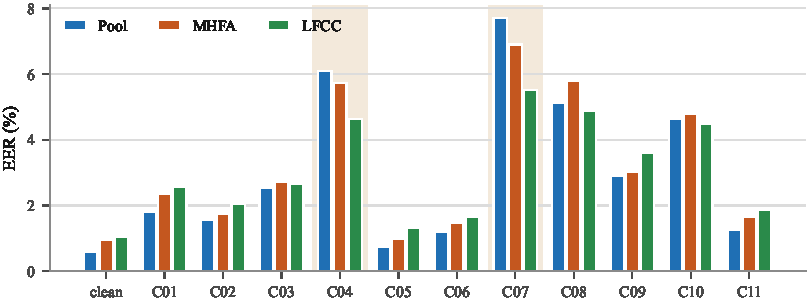
\includegraphics[width=\textwidth]{figures/fig4_per_codec}
\caption{Per-condition \eer{}. The neural codecs C04 and C07 (shaded) are the hardest conditions for
every member, and the development split contains neither.}
\label{fig:codec}
\end{figure}

\subsection{How many systems is a four-member ensemble?}
\label{sec:rank}

\begin{figure}[t]
\centering
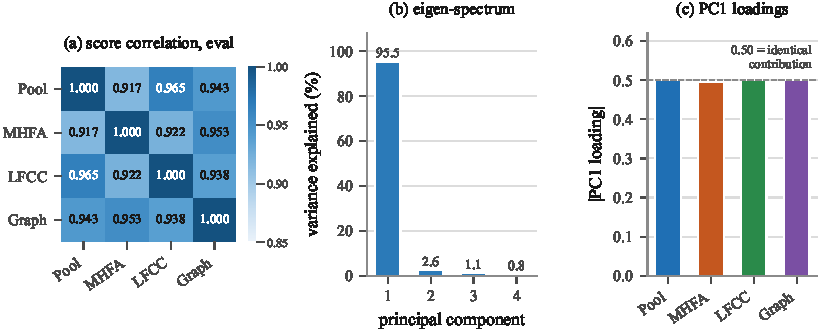
\includegraphics[width=\textwidth]{figures/fig6_spectrum}
\caption{(a) Score correlation on the evaluation set. (b) Eigen-spectrum of that matrix: the first
component explains 95.5\% of the variance. (c) Its loadings are within 0.006 of $0.50$ on every
member---the first component \emph{is} the unweighted mean.}
\label{fig:spectrum}
\end{figure}

We summarise a member set by the eigen-spectrum of its score correlation matrix, reporting the
participation ratio $(\sum_i \lambda_i)^2 / \sum_i \lambda_i^2$ and the entropy rank
$\exp(-\sum_i p_i \log p_i)$ with $p_i = \lambda_i / \sum_j \lambda_j$. Both equal $1$ when all
members are the same system and $M$ when they are orthogonal.

Figure~\ref{fig:spectrum} gives the answer: \textbf{1.10 effective systems out of four}
(entropy rank 1.26), with PC1 explaining 95.5\% of the variance and loading
$0.501, 0.496, 0.501, 0.502$. On the out-of-domain set the figure is 1.15 of 4. Changing the
pooling, the representation, the topology \emph{and} the backbone moves the effective rank by
0.1.

This reframes the fusion question. Table~\ref{tab:selection} shows the gain available: the best
two-member fusion improves on its best member by 0.18~\eer{} points, and a third member adds
nothing. The relevant comparison is \citet{ustc2024}, whose twelve systems across three back-end
families gain 35\% relative from fusion. Our members do not differ enough for that mechanism to
engage, and the axis that moved them at all was the one that changed what the model \emph{sees},
not how it is parameterised: replacing time-mean pooling with attention over frames took the
correlation from 0.994 (for a member differing only in augmentation strength) to 0.917.

\subsection{Selection fails, and we report both numbers}
\label{sec:selection}

\begin{table}[t]
\centering
\small
\caption{Member subsets ranked by development \eer{}, top four of fifteen, plus the best subset on
evaluation. The protocol selects row~1. The oracle row is shown for comparison and is \emph{not}
claimed as a result.}
\label{tab:selection}
\begin{tabular}{llrrrr}
\toprule
Rank & Subset & Dev sel. & eval \eer{} & eval \mindcf{} & ITW \eer{} \\
\midrule
\multicolumn{6}{l}{\emph{Selection on clean + codec ($\rho=+0.011$, $p=0.97$)}}\\
1 & Pool + MHFA          & \best{1.46} & 3.21 & 0.0905 & 9.04 \\
2 & Pool                 & 1.47 & 3.31 & 0.0942 & 11.25 \\
3 & Pool + MHFA + Graph  & 1.67 & 3.20 & 0.0903 & 8.80 \\
4 & Pool + MHFA + LFCC   & 1.72 & 2.94 & 0.0827 & 9.04 \\
7 & \emph{Pool + LFCC} (oracle) & 1.83 & \emph{2.93} & \emph{0.0819} & 9.19 \\
\midrule
\multicolumn{6}{l}{\emph{Selection with a neural-codec view added ($\rho=+0.236$, $p=0.40$)}}\\
1 & Pool + MHFA          & \best{2.79} & 3.21 & 0.0905 & 9.04 \\
2 & Pool + MHFA + LFCC   & 2.90 & 2.94 & 0.0827 & 9.04 \\
6 & \emph{Pool + LFCC} (oracle) & 3.01 & \emph{2.93} & \emph{0.0819} & 9.19 \\
\bottomrule
\end{tabular}
\end{table}

\begin{figure}[t]
\centering
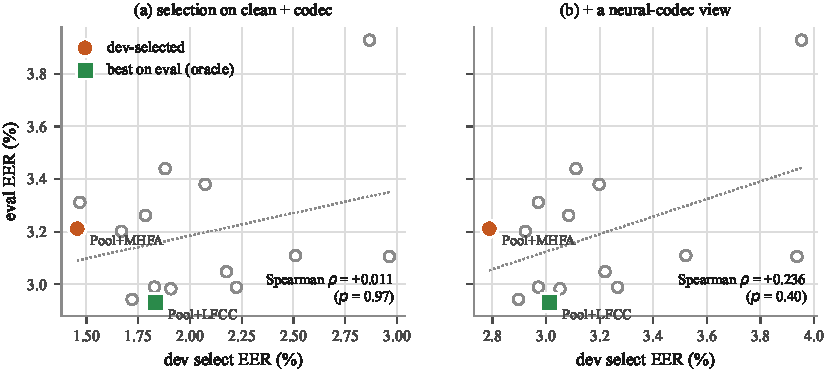
\includegraphics[width=\textwidth]{figures/fig7_selection}
\caption{Development \eer{} against evaluation \eer{} for all 15 member subsets. The dotted line is
a least-squares fit. Adding a neural-codec view to the selection set improves the ordering---the
three-member system climbs from rank 4 to rank 2---but does not make it predictive.}
\label{fig:selection}
\end{figure}

Over all 15 subsets the rank correlation between development and evaluation \eer{} is
$\rho = +0.011$ ($p=0.97$): the development split carries \emph{no} information about evaluation
ordering (Figure~\ref{fig:selection}a). Since the evaluation set's discriminating conditions are
real codecs and the development split has none, we scored every member through an added
neural-codec development view. This helps---the three-member system climbs from rank 4 to rank 2,
and $\rho$ rises to $+0.236$---but at $p=0.40$ it is still not distinguishable from zero
(Figure~\ref{fig:selection}b).

The consequence is Table~\ref{tab:selection}. Our protocol selects Pool\,+\,MHFA at
\textbf{3.21\% / 0.0905}. The best system in our pool is Pool\,+\,LFCC at \emph{2.93\% / 0.0819},
which the protocol ranks seventh of fifteen. \textbf{We report the first as our result and the second
as an oracle bound, and we take the 0.28-point gap between them to be a measurement of the selection
set rather than a property of our models.} We are not aware of a prior quantification of this gap on
ASVspoof~5.

\subsection{In-domain and out-of-domain rankings invert}

\begin{figure}[t]
\centering
\begin{minipage}{0.48\textwidth}
\centering
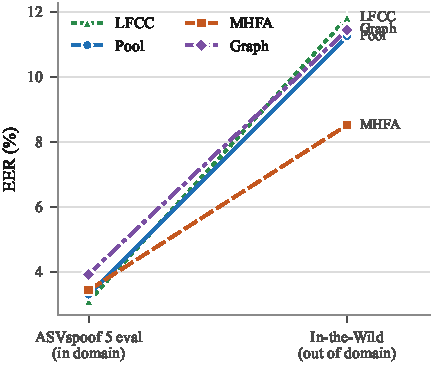
\includegraphics[width=\textwidth]{figures/fig8_transfer}
\end{minipage}\hfill
\begin{minipage}{0.48\textwidth}
\centering
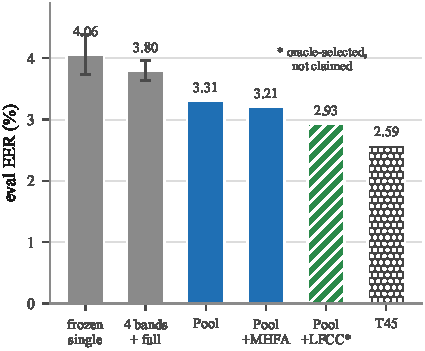
\includegraphics[width=\textwidth]{figures/fig9_progress}
\end{minipage}
\caption{Left: every system degrades by 2.5--3.8$\times$ out of domain, and the ordering inverts.
Right: progression of this work. Bars with error bars are three-seed means with spread; the
remainder are single-seed. The hatched bar is oracle-selected and not claimed.}
\label{fig:transfer}
\end{figure}

Figure~\ref{fig:transfer} (left) plots each member in domain and out. Every system loses a factor of
2.5--3.8, which is in line with the literature. What is not routine is the inversion: LFCC, our best
in-domain member at 3.11\%, is our worst in the wild at 11.82\%, while MHFA goes from third
(3.44\%) to first (8.51\%), a 24\% relative margin over the next system.

A plausible reading is that cepstral evidence is partly \emph{channel} evidence, and channel
statistics are exactly what does not transfer from a single curated corpus to found audio, whereas
attentive pooling over time learns something less corpus-specific. We offer this as a hypothesis;
our experiments establish the inversion, not its cause.

The practical implication is uncomfortable for leaderboard optimisation. Pursuing the final
0.6~\eer{} points in domain would mean preferring exactly the member that transfers worst.

\subsection{Adversarial robustness}
\label{sec:robust}

\begin{table}[t]
\centering
\small
\caption{Attack success at a 0.1\% false-alarm operating point, 20-step PGD under an SNR-constrained
$L_2$ budget; realised SNR is reported, not assumed. Four defence routes are closed. The fifth,
waveform adversarial training, was still training at submission.}
\label{tab:robust}
\begin{tabular}{llrrr}
\toprule
Defence & Attack & Clean \eer{} & 30\,dB & 20\,dB \\
\midrule
single model            & white-box PGD & 4.78 & 1.000 & 1.000 \\
single model            & SPSA, 320 queries & 4.78 & --- & 0.011 \\
four layer bands        & white-box PGD & 4.78 & 1.000 & 1.000 \\
four layer bands        & transfer PGD  & 4.78 & 1.000 & 1.000 \\
WavLM, surrogate XLS-R  & transfer PGD  & 4.78 & 0.892 & 0.995 \\
XLS-R, surrogate WavLM  & transfer PGD  & 9.21 & 0.832 & 0.984 \\
feature-space adv.\ training & white-box PGD & 13.95 & 0.993 & 1.000 \\
feature-space adv.\ training & transfer PGD  & 13.95 & 0.776 & 0.977 \\
\bottomrule
\end{tabular}
\end{table}

Table~\ref{tab:robust} summarises the robustness measurements. A gradient-bearing attacker succeeds
on essentially every clip at perturbations of 30\,dB SNR, for every defence we tried: a single model,
a four-member band ensemble, across two different SSL backbones, and after feature-space adversarial
training---which additionally destroyed clean accuracy (13.95\% \eer{}). A query-limited black-box
attacker with 320 queries per clip succeeds on about 1\%.

We flag one methodological point about the feature-space row. That defence hardened the \emph{head}
against perturbations in \emph{feature} space, while the attacker perturbs the \emph{waveform} and
arrives through the backbone. The mismatch means its failure is weak evidence: it does not show that
adversarial training fails here, only that this version of it answers a different question. A
waveform-domain run---half of each batch replaced by 30\,dB PGD examples crafted through the
backbone---was still training at submission and is reported as AdvWav in Figure~\ref{fig:curves}.

\section{Limitations}

We state these rather than leave them to be found.

\textbf{Single seed.} Every system in Table~\ref{tab:members} is one seed. Three-seed experiments
earlier in this work gave a spread of 0.33~\eer{} points on frozen single models, larger than the
0.10-point fusion gain. The fusion gain is therefore not established against seed variance.

\textbf{One corpus.} We train on ASVspoof~5 alone. The system we compare against \citep{ustc2024}
trains on four corpora. We cannot separate ``our architecture is worse'' from ``our supervision is
narrower''.

\textbf{Clustered intervals matter.} Section~\ref{sec:data} shows that clip-level bootstrap
intervals on this corpus are about $2\times$ too narrow. Our conclusions survive the correction
because the differences we claim are many standard errors wide, but intervals reported elsewhere on
this corpus may not.

\textbf{One out-of-domain set.} In-the-Wild has its own biases---public figures, internet audio, an
inverted class prior. One such set measures a gap; it does not characterise generalisation.

\textbf{The graph member is not AASIST} and must not be cited as evidence about AASIST.

\section{Conclusion}

Four detectors differing in pooling, representation, topology and backbone amount to 1.10
independent systems. Architectural variety is not the same as error diversity, and only a change in
what the model \emph{sees} moved the correlation at all. Meanwhile the development split of the
corpus everyone uses cannot rank these systems, costing our protocol 0.28~\eer{} points against its
own oracle; and in-domain ranking inverts out of domain, so the member that wins the leaderboard is
the one that transfers worst.

Our selected system reaches 3.21\% \eer{} / 0.0905 \mindcf{}, ahead of the other published
open-condition system we were able to verify \citep[4.04\% / 0.115]{szuafs} and short of the
twelve-system winner at 2.59\% / 0.0750 \citep{ustc2024}. A further comparison point of 4.17\% /
0.119 for the best single system appears in our own experiment log, but we could not verify its
source at the time of writing and therefore do not rely on it~[CITATION NEEDED]. We think the more
useful contribution is the measurement around that number: a reproducible way to ask how many systems
an ensemble really contains, and evidence that the standard selection procedure on this benchmark
does not work.

\section*{Reproducibility}

Figures are generated by \texttt{paper/make\_figures.py} from a single JSON of measured values, so no
number in the text can disagree with a figure. Every experiment, including the failures and the
predictions that turned out wrong, is recorded in \texttt{docs/experiment\_log.md}.

\bibliographystyle{plainnat}
\bibliography{refs}

\end{document}
